%!TEX program = xelatex
\PassOptionsToPackage{full}{textcomp}
\documentclass[lang=en,11pt,a4paper,citestyle =authoryear]{elegantpaper}

% 标题
\title{HW2 - STAT 701}
\author{Wells Guan}

% 本文档命令
\usepackage{array,url,stix}
\usepackage{tikz}
\usepackage{tikz-cd}
\usepackage{enumitem}
\usepackage{amsmath}
\usepackage{amssymb}
\usepackage{listings}
\usepackage{subfigure}

\lstset{
    frame=single,
    columns=fullflexible,
    keepspaces=true,
    showstringspaces=false,
    breaklines=true,
    breakatwhitespace=false,
    basicstyle=\ttfamily\footnotesize,
    numbers=left,
    numberstyle=\tiny,
    numbersep=6pt
}
\newcommand{\ccr}[1]{\makecell{{\color{#1}\rule{1cm}{1cm}}}}
\newcommand{\code}[1]{\lstinline{#1}}
\newcommand{\prvd}{$\hfill \qedsymbol$}
\newcommand{\Z}{\mathbb{Z}}
\newcommand{\R}{\mathbb{R}}
\newcommand{\N}{\mathbb{N}}
\newcommand{\C}{\mathbb{C}}
\newcommand{\Q}{\mathbb{Q}}
\newcommand{\M}{\mathcal{M}}
\newcommand{\B}{\mathcal{B}}
\newcommand{\X}{\mathcal{X}}
\newcommand{\Hil}{\mathcal{H}}
\newcommand{\range}{\mathcal{R}}
\newcommand{\nul}{\mathcal{N}}

% 文档区
\begin{document}
\maketitle

\noindent The appendix contains the Python source used for all simulations,
estimation, diagnostics, and figures. The source files contain no inline
comments.

\subsection*{Problem 1. Textbook exercises}
Brockwell and Davis 3.1, 3.11, 4.8, 4.13. For 3.1, you are welcome to check for causality/invertibility with the assistance of a computer in the sense of using a computer program to compute, e.g., roots of a polynomial. You are not welcome to find some package that offers a function where you just dump in coefficients and get back the answer.

\subsubsection*{Ex. 3.1}
Determine which of the following processes are causal and/or invertible:
\begin{enumerate}[label=(\alph*),leftmargin=*]
    \item $X_t+.2X_{t-1}-.48X_{t-2}=Z_t$;
    \item $X_t+1.9X_{t-1}+.88X_{t-2}
    =Z_t+.2Z_{t-1}+.7Z_{t-2}$;
    \item $X_t+.6X_{t-2}=Z_t+1.2Z_{t-1}$;
    \item $X_t+1.8X_{t-1}+.81X_{t-2}=Z_t$;
    \item $X_t+1.6X_{t-1}=Z_t-.4Z_{t-1}+.04Z_{t-2}$.
\end{enumerate}
\par\vspace{0.5em}
\textbf{Sol.}\par
Write each equation as
\[
\phi(B)X_t=\theta(B)Z_t.
\]
Since the AR and MA polynomials below have no common zeroes, the process is
causal if and only if every zero of $\phi$ lies outside the closed unit disk,
and it is invertible if and only if every zero of $\theta$ lies outside the
closed unit disk.
\begin{enumerate}[label=(\alph*),leftmargin=*]
    \item We have
    \[
    \phi(z)=1+.2z-.48z^2=(1-.6z)(1+.8z),
    \qquad \theta(z)=1.
    \]
    The zeroes of $\phi$ are $5/3$ and $-5/4$, both of which have
    modulus greater than $1$. Since $\theta$ has no zeroes, the process is
    both causal and invertible.

    \item Here
    \[
    \phi(z)=1+1.9z+.88z^2=(1+1.1z)(1+.8z),
    \qquad \theta(z)=1+.2z+.7z^2.
    \]
    The zeroes of $\phi$ are $-10/11$ and $-5/4$. Since
    $|-10/11|<1$, the process is not causal. The two zeroes of $\theta$
    are complex conjugates, and their common modulus is
    \[
    \sqrt{\frac{1}{.7}}=\sqrt{\frac{10}{7}}>1.
    \]
    Hence the process is invertible.

    \item We have
    \[
    \phi(z)=1+.6z^2,
    \qquad \theta(z)=1+1.2z.
    \]
    The zeroes of $\phi$ are $\pm i\sqrt{5/3}$, whose modulus is greater
    than $1$, so the process is causal. The zero of $\theta$ is $-5/6$,
    which lies inside the unit disk, so the process is not invertible.

    \item Here
    \[
    \phi(z)=1+1.8z+.81z^2=(1+.9z)^2,
    \qquad \theta(z)=1.
    \]
    The only zero of $\phi$ is $-10/9$, with multiplicity two, and it lies
    outside the unit disk. Thus the process is both causal and invertible.

    \item Finally,
    \[
    \phi(z)=1+1.6z,
    \qquad
    \theta(z)=1-.4z+.04z^2=(1-.2z)^2.
    \]
    The zero of $\phi$ is $-5/8$, so the process is not causal. The only
    zero of $\theta$ is $5$, with multiplicity two, so the process is
    invertible.
\end{enumerate}
\vspace{1em}

\subsubsection*{Ex. 3.11}
Let $\{X_t\}$ be an ARMA process with $\phi(z)\neq 0$ for $|z|=1$
and autocovariance function $\gamma(\cdot)$. Show that there exist constants
$C>0$ and $s\in(0,1)$ such that
\[
|\gamma(h)|\leq Cs^{|h|},\qquad h=0,\pm1,\ldots,
\]
and hence that
\[
\sum_{h=-\infty}^{\infty}|\gamma(h)|<\infty.
\]
\par\vspace{0.5em}
\textbf{Sol.}\par
Let $\sigma^2$ be the white-noise variance. On the unit circle, the spectral
density of $\{X_t\}$ is
\[
f(\lambda)=\frac{\sigma^2}{2\pi}
\frac{\theta(e^{-i\lambda})\theta(e^{i\lambda})}
     {\phi(e^{-i\lambda})\phi(e^{i\lambda})}.
\]
Consider the rational function
\[
F(z)=\sigma^2
\frac{\theta(z)\theta(z^{-1})}
     {\phi(z)\phi(z^{-1})}.
\]
Because $\phi$ has only finitely many zeroes and none lies on the unit
circle, there are numbers $r<1<R$ such that $F$ is analytic on the annulus
\[
r<|z|<R.
\]
Hence $F$ has a Laurent expansion there,
\[
F(z)=\sum_{h=-\infty}^{\infty}a_hz^h.
\]
The Fourier inversion formula on $|z|=1$ shows that, up to reversing the
index according to the Fourier convention, these Laurent coefficients are
the autocovariances. Since $\gamma(-h)=\gamma(h)$, we may write
$|a_h|=|\gamma(h)|$.

Choose $r<r_0<1<R_0<R$, and set
\[
M_+=\max_{|z|=R_0}|F(z)|,
\qquad
M_- =\max_{|z|=r_0}|F(z)|.
\]
The Cauchy estimates for Laurent coefficients give, for $h\geq 0$,
\[
|a_h|\leq M_+R_0^{-h},
\qquad
|a_{-h}|\leq M_-r_0^h.
\]
Let
\[
s=\max\{R_0^{-1},r_0\}<1,
\qquad
C=\max\{M_+,M_-\}.
\]
It follows that
\[
|\gamma(h)|\leq Cs^{|h|},
\qquad h\in\mathbb Z.
\]
Finally,
\[
\sum_{h=-\infty}^{\infty}|\gamma(h)|
\leq C\sum_{h=-\infty}^{\infty}s^{|h|}
=C\left(1+2\sum_{h=1}^{\infty}s^h\right)
=C\frac{1+s}{1-s}<\infty.
\]
\vspace{1em}

\subsubsection*{Ex. 4.8}
Let $\{X_t\}$ and $\{Y_t\}$ be stationary zero-mean processes with spectral
densities $f_X$ and $f_Y$. If
\[
f_X(\lambda)\leq f_Y(\lambda)
\qquad\text{for all }\lambda\in[-\pi,\pi],
\]
show that
\begin{enumerate}[label=(\alph*),leftmargin=*]
    \item $\Gamma_{n,Y}-\Gamma_{n,X}$ is a non-negative definite matrix,
    where $\Gamma_{n,Y}$ and $\Gamma_{n,X}$ are the covariance matrices of
    $\mathbf Y=(Y_1,\ldots,Y_n)'$ and
    $\mathbf X=(X_1,\ldots,X_n)'$, respectively; and
    \item $\operatorname{Var}(\mathbf b'\mathbf X)
    \leq\operatorname{Var}(\mathbf b'\mathbf Y)$ for all
    $\mathbf b=(b_1,\ldots,b_n)'\in\mathbb R^n$.
\end{enumerate}
\par\vspace{0.5em}
\textbf{Sol.}\par
For any $\mathbf b=(b_1,\ldots,b_n)'\in\mathbb R^n$, stationarity and the
spectral representation of the autocovariance function give
\begin{align*}
\mathbf b'\Gamma_{n,X}\mathbf b
&=\sum_{j=1}^n\sum_{k=1}^n b_jb_k\gamma_X(j-k)\\
&=\int_{-\pi}^{\pi}
  \left|\sum_{j=1}^n b_je^{ij\lambda}\right|^2
  f_X(\lambda)\,d\lambda.
\end{align*}
The same identity holds for $Y$. Therefore
\begin{align*}
\mathbf b'(\Gamma_{n,Y}-\Gamma_{n,X})\mathbf b
&=\int_{-\pi}^{\pi}
  \left|\sum_{j=1}^n b_je^{ij\lambda}\right|^2
  \bigl(f_Y(\lambda)-f_X(\lambda)\bigr)\,d\lambda\\
&\geq 0,
\end{align*}
because both factors in the integrand are non-negative. This holds for every
$\mathbf b\in\mathbb R^n$, so
$\Gamma_{n,Y}-\Gamma_{n,X}$ is non-negative definite, proving (a).

Since the processes have mean zero,
\[
\operatorname{Var}(\mathbf b'\mathbf X)
=\mathbf b'\Gamma_{n,X}\mathbf b,
\qquad
\operatorname{Var}(\mathbf b'\mathbf Y)
=\mathbf b'\Gamma_{n,Y}\mathbf b.
\]
The inequality just established thus immediately yields
\[
\operatorname{Var}(\mathbf b'\mathbf X)
\leq \operatorname{Var}(\mathbf b'\mathbf Y),
\]
which proves (b).
\vspace{1em}

\subsubsection*{Ex. 4.13}
If $\{X_t\}$ and $\{Y_t\}$ are stationary processes satisfying
\[
X_t-\alpha X_{t-1}=W_t,
\qquad \{W_t\}\sim\operatorname{WN}(0,\sigma^2),
\]
and
\[
Y_t-\alpha Y_{t-1}=X_t+Z_t,
\qquad \{Z_t\}\sim\operatorname{WN}(0,\sigma^2),
\]
where $|\alpha|<1$ and $\{W_t\}$ and $\{Z_t\}$ are uncorrelated, find the
spectral density of $\{Y_t\}$.
\par\vspace{0.5em}
\textbf{Sol.}\par
Using the backshift operator $B$, the first equation gives
\[
X_t=\frac{1}{1-\alpha B}W_t.
\]
Substituting this into the second equation yields
\begin{align*}
Y_t
&=\frac{1}{1-\alpha B}(X_t+Z_t)\\
&=\frac{1}{(1-\alpha B)^2}W_t
  +\frac{1}{1-\alpha B}Z_t.
\end{align*}
Because $|\alpha|<1$, both filters are stable. Moreover, $\{W_t\}$ and
$\{Z_t\}$ are uncorrelated, so the two filtered processes above have zero
cross-spectrum. Their spectral densities therefore add, giving
\begin{align*}
f_Y(\lambda)
&=\frac{\sigma^2}{2\pi}
  \left(
  \frac{1}{|1-\alpha e^{-i\lambda}|^4}
  +\frac{1}{|1-\alpha e^{-i\lambda}|^2}
  \right)\\
&=\frac{\sigma^2}{2\pi}
  \frac{2+\alpha^2-2\alpha\cos\lambda}
       {(1+\alpha^2-2\alpha\cos\lambda)^2},
\qquad -\pi\leq\lambda\leq\pi,
\end{align*}
where we used
\[
|1-\alpha e^{-i\lambda}|^2
=1+\alpha^2-2\alpha\cos\lambda.
\]
\vspace{1em}

\newpage
\subsection*{Problem 2.}
An ARIMA$(p,d,q)$ (where the I is for \textit{integrated}) process is a time series $\{X_t\}$ where $(I-B)^dX_t$ is an ARMA$(p,q)$ process. A SARIMA$(s,p,d,q)$, where the S is for \textit{seasonal}, process is a time series where $(I-B^s)X_t$ is an ARIMA$(p,d,q)$ process. Let's explore simulating and fitting these extensions to data. For this question, you are welcome to find a package that fits (S)AR(I)MA models, but find one that lets you specify the degrees $s,p,d,q$ manually! We'll talk about estimation in detail later in the semester, but I don't want to wait too long before asking you to start connecting the math to data.

\begin{enumerate}[label=\arabic*.,leftmargin=*]
\item Write a function in whatever programming language you like to simulate an ARMA$(p,q)$ process in the state-space formulation. Importantly, please design this program to accept custom white noise generators. For a Gaussian white noise, generate a length $n=1{,}000$ ARMA$(p,q)$ process with, say, $p,q>3$ and put it into the estimation function that you find to check your work.
\par\vspace{0.5em}\textbf{Sol.}\par
I used the convention
\[
X_t=\sum_{j=1}^p\phi_jX_{t-j}+Z_t+
\sum_{j=1}^q\theta_jZ_{t-j}.
\]
If
\[
\mathbf s_t=(X_t,\ldots,X_{t-p+1},Z_t,\ldots,Z_{t-q+1})',
\]
then this recursion has the state-space form
\[
\mathbf s_t=A\mathbf s_{t-1}+\mathbf gZ_t,
\]
where the first row of $A$ is
$(\phi_1,\ldots,\phi_p,\theta_1,\ldots,\theta_q)$, the remaining rows shift
the stored observations and innovations by one coordinate, and $\mathbf g$
has ones in coordinates $1$ and $p+1$ and zeroes elsewhere. The function in
the appendix implements this update and receives the innovation generator as
an argument.

I simulated an ARMA$(4,4)$ process with
\[
\boldsymbol\phi=(.8,-.3,.1,-.05),
\qquad
\boldsymbol\theta=(-.6,.2,.1,.05),
\qquad Z_t\sim N(0,1),
\]
discarding a burn-in of $1{,}000$ observations. I then fitted an
ARMA$(4,4)$ model with the standard Gaussian maximum-likelihood routine in
\texttt{statsmodels}. The estimates were
\[
\widehat{\boldsymbol\phi}=(.7469,-.0024,.0185,-.1247),
\qquad
\widehat{\boldsymbol\theta}=(-.5926,-.0418,.1559,.0776),
\]
with $\widehat\sigma^2=1.0179$. The leading AR and MA effects and the
innovation variance are recovered well. Individual higher-order
coefficients are less precisely identified from only $1{,}000$ observations,
which is common for a deliberately high-order ARMA model.

\begin{figure}[htbp]
    \centering
    \graphicspath{{png/}{STATS_Minor/701/HW2/png/}}
    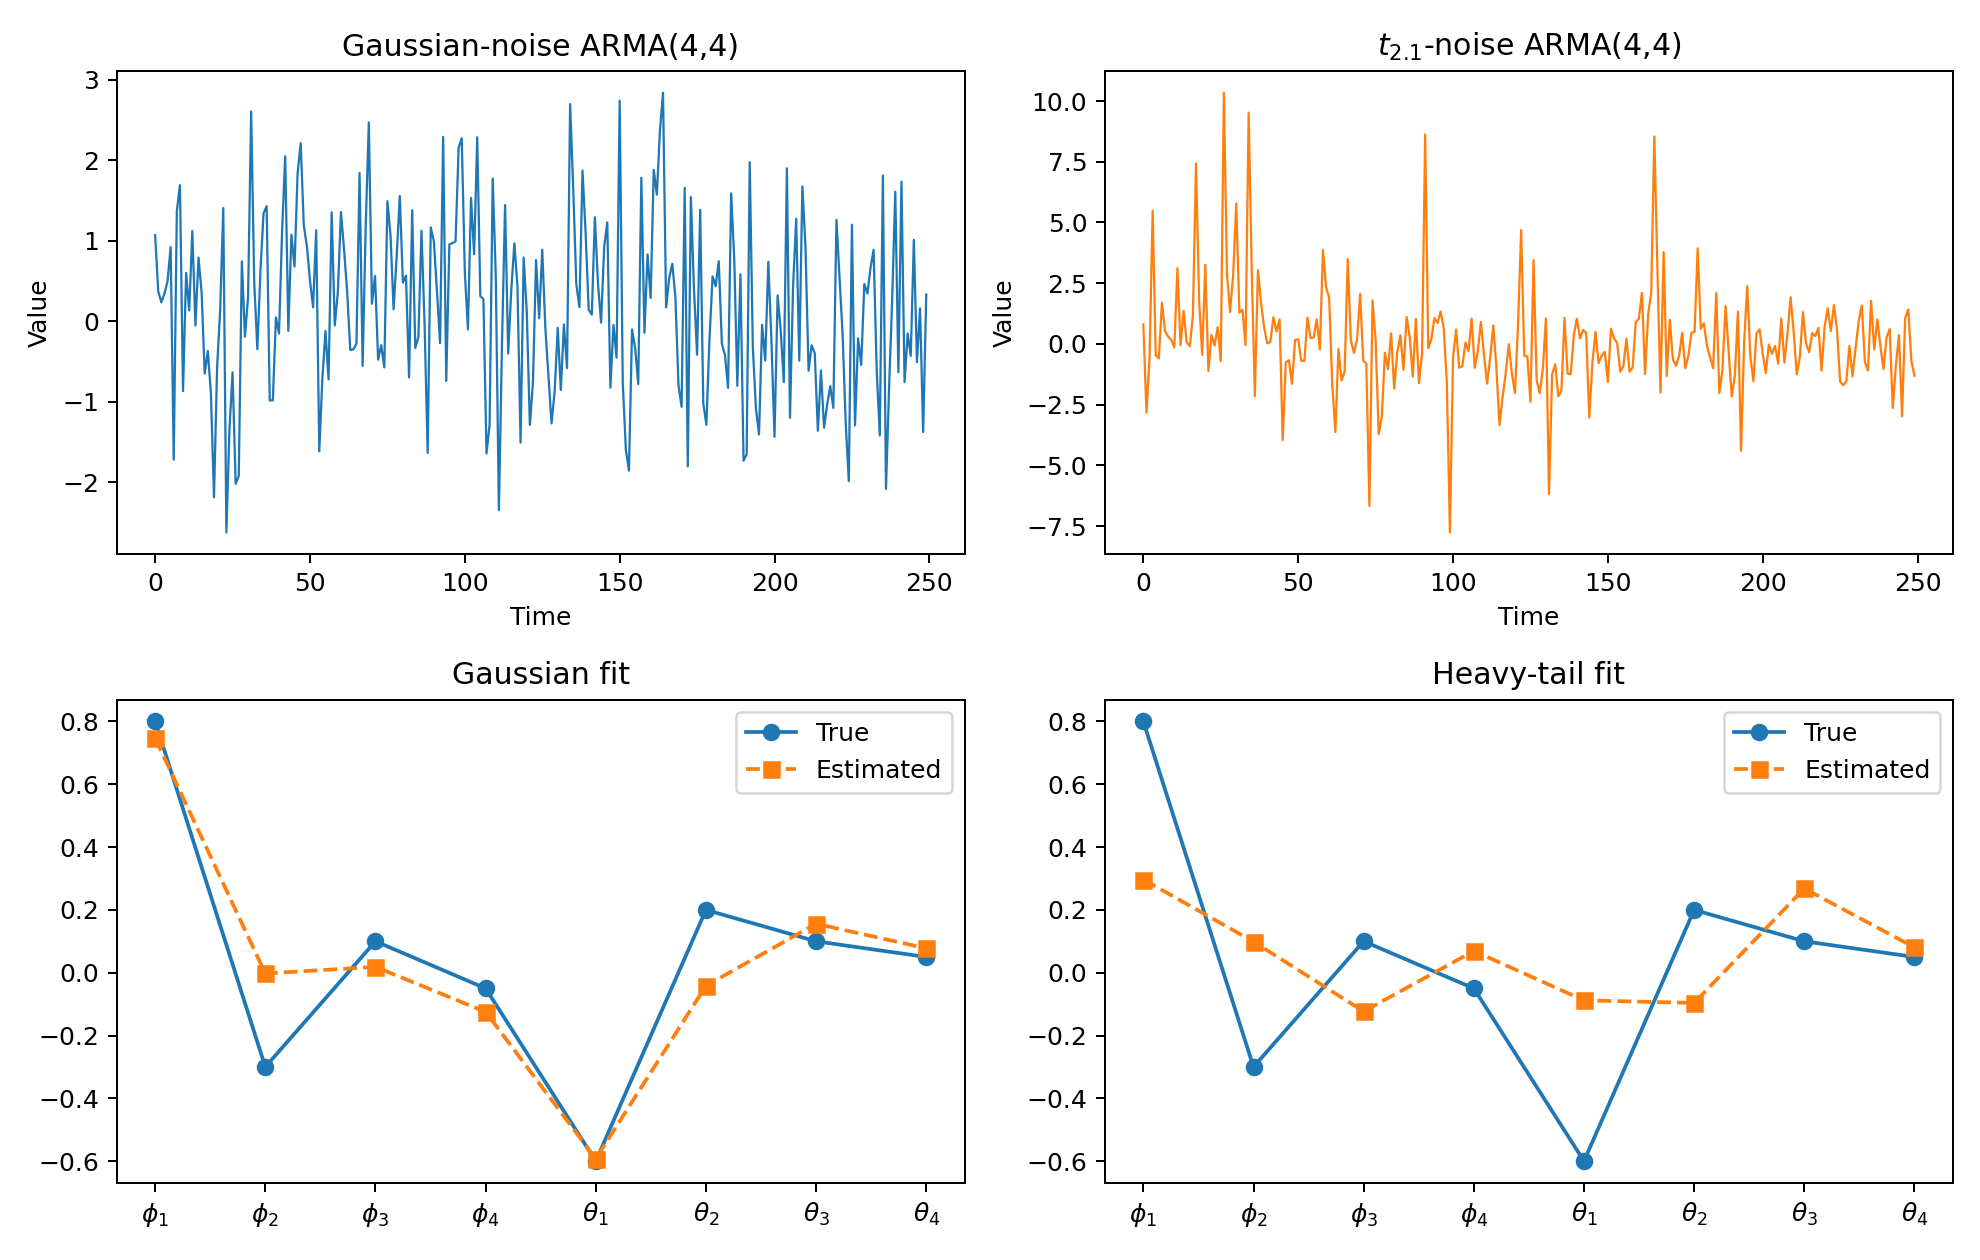
\includegraphics[width=0.95\linewidth]{problem2_arma_fits.png}
    \caption{Gaussian and heavy-tailed ARMA simulations and fitted coefficients.}
\end{figure}
\vspace{1em}

\item Now, using the same coefficients, generate a similar length dataset but with $Z_t\sim t_{2.1}$ (the t-distribution with $\nu=2.1$ degrees of freedom). Run it through your estimation function again and comment on your results. How would you summarize the effect of very heavy tailed noise on generic estimation packages?
\par\vspace{0.5em}\textbf{Sol.}\par
Using the same state transition and replacing only the innovation generator by
$t_{2.1}$ gave
\[
\widehat{\boldsymbol\phi}=(.2967,.0987,-.1233,.0692),
\qquad
\widehat{\boldsymbol\theta}=(-.0880,-.0963,.2682,.0805),
\]
and $\widehat\sigma^2=104.2024$. For comparison, a $t_{2.1}$ variable has
variance $2.1/(2.1-2)=21$, but its fourth moment is infinite. Thus even a
sample of length $1{,}000$ can contain a few observations that dominate the
Gaussian likelihood and make the sample variance far larger than its
population value. Figure 1 shows the resulting isolated spikes and the
substantial coefficient distortion. Generic Gaussian ARMA estimators can
therefore be highly unstable under very heavy tails: the estimated innovation
variance is especially sensitive, standard errors based on Gaussian moments
are unreliable, and the dynamic coefficients may shift to accommodate a few
extreme observations. Robust likelihoods or estimators designed for heavy
tails are preferable in this setting.
\vspace{1em}

\item Download \texttt{nao.csv}, the North Atlantic Oscillation time series from Canvas (and note there is a missing value, which you'll have to decide how to address). Using empirical ACFs and pACFs like I quickly demonstrated in class (both on your data and on differenced data and so on), do some exploratory analysis and propose and fit a SARIMA$(s,p,d,q)$ model. Please report your final model and provide justification for your choices. As a final validation, please simulate from your model and repeat the diagnostics on your simulated data. Discuss your results. In particular, try to propose the most important feature of this data that your SARIMA model is not capturing.
\par\vspace{0.5em}\textbf{Sol.}\par
The supplied file contains $17{,}410$ daily observations from 1979 through
August 2026. Although the filename is \texttt{nao.csv}, its value column is
labelled \texttt{aao\_index\_cdas}; all calculations below use the supplied
column as given. The only missing observation is April 30, 2003. I replaced it
by linear interpolation between the adjacent days.

The raw ACF is .9512 at lag 1, .8488 at lag 2, .4837 at lag 7, and .1132 at
lag 30. It is only $-.0289$ at lag 365, so the annual component is much weaker
than the short-range persistence. Nevertheless, because the observations are
daily and the requested model is seasonal, I used $s=365$. After applying
$1-B^{365}$, the pACF has its main values at lags 1 through 5 and is close to
zero thereafter, while the ACF decays gradually. This led to the parsimonious
choice SARIMA$(365,4,0,2)$:
\[
(1-.6642B-.3518B^2+.2324B^3-.0837B^4)(1-B^{365})X_t
=(1+1.1556B+.3247B^2)Z_t,
\]
with estimated innovation variance $\widehat\sigma^2=.1956$.

\begin{figure}[htbp]
    \centering
    \graphicspath{{png/}{STATS_Minor/701/HW2/png/}}
    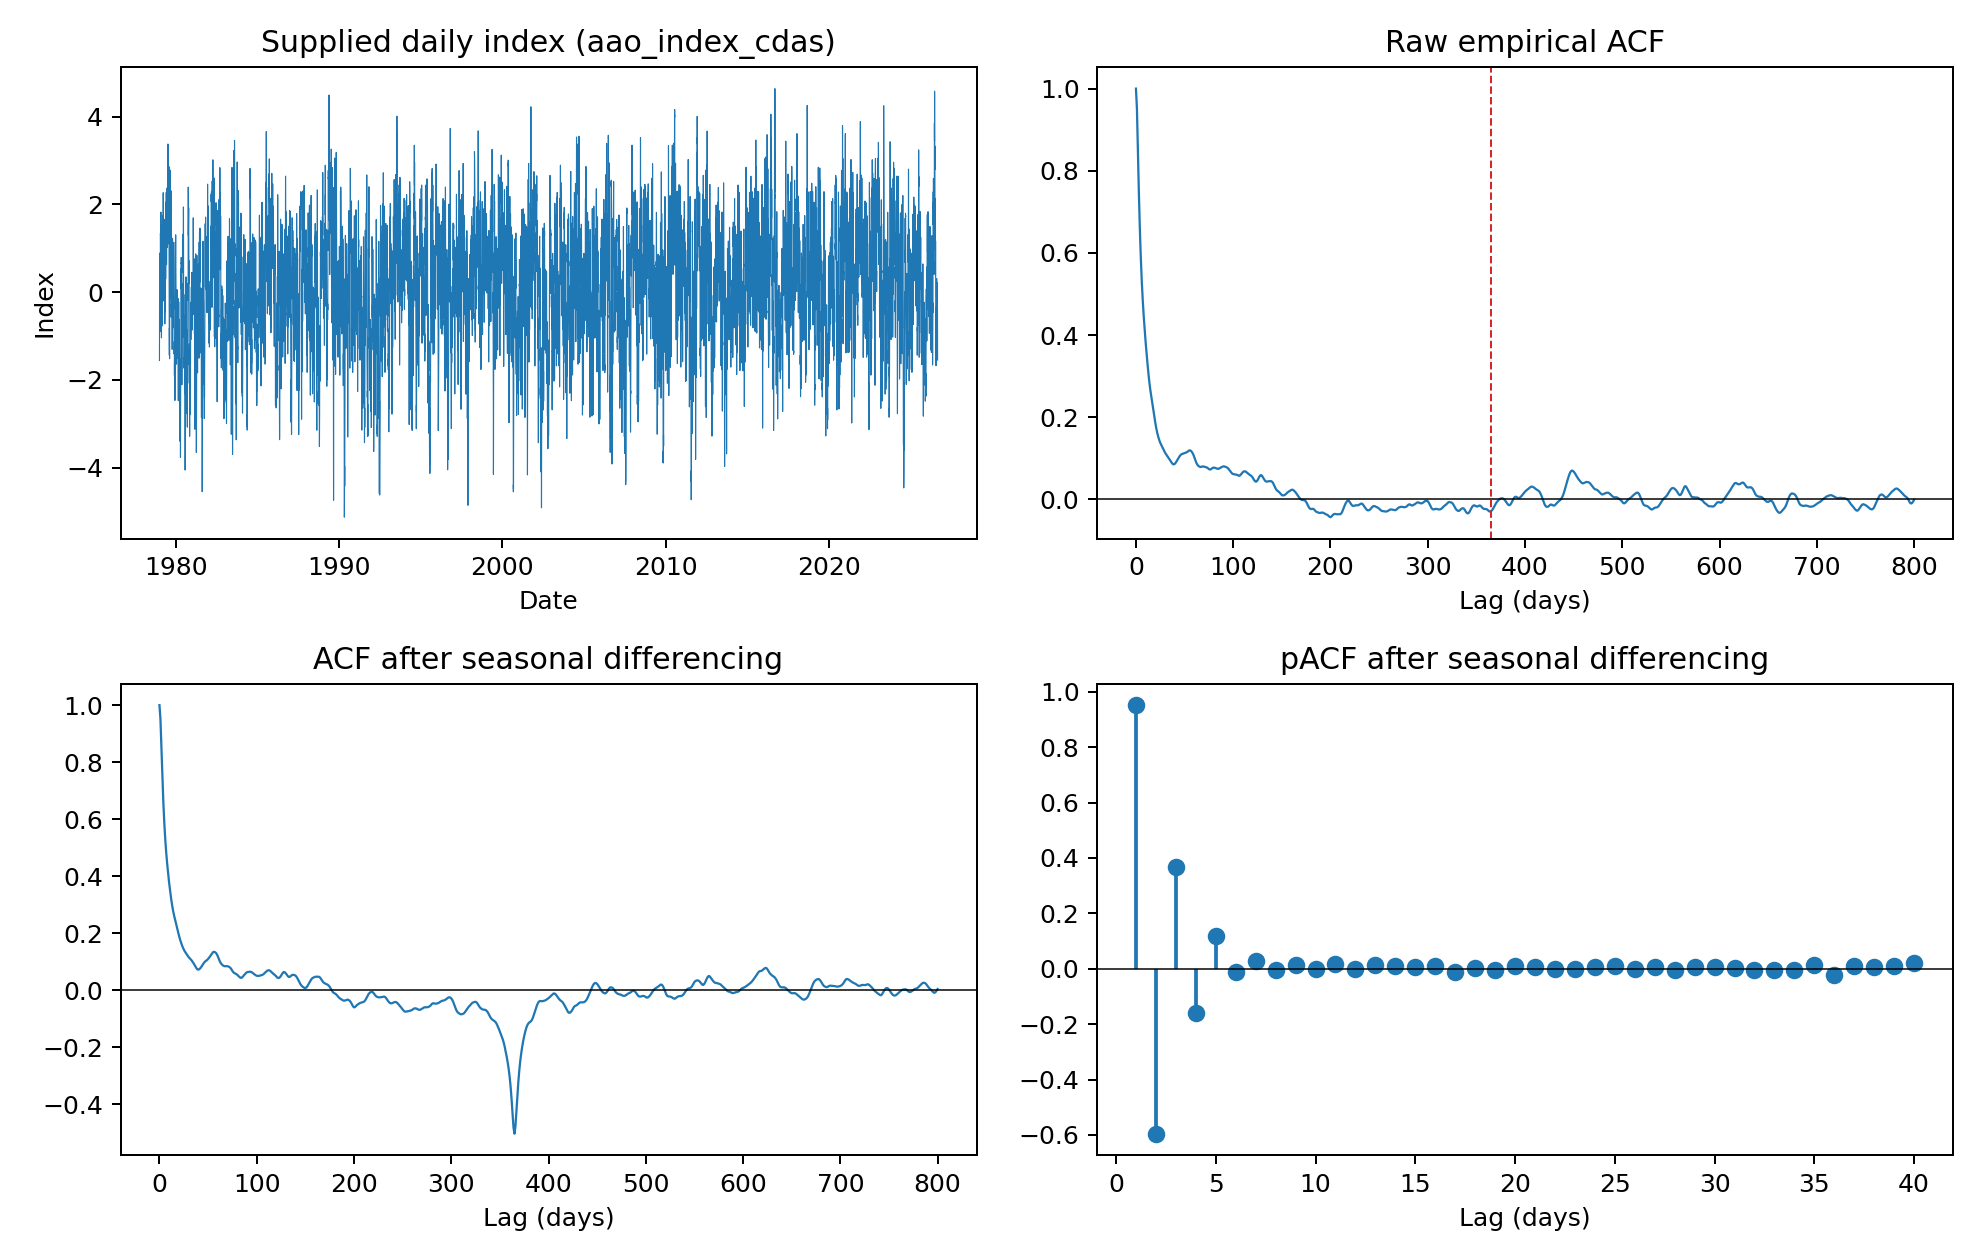
\includegraphics[width=0.95\linewidth]{problem2_nao_diagnostics.png}
    \caption{The supplied index and empirical ACF/pACF diagnostics.}
\end{figure}

I simulated the fitted ARMA equation for the seasonally differenced series and
then reconstructed a series recursively from its first $365$ values. The
short-lag ACF of the simulated differences is close to the observed one, and
the fitted residual correlations are all below .027 in magnitude. The model
does not reproduce the slower positive ACF extending across several dozen
days, and several residual correlations exceed the approximate 95\% bounds.
The main omitted feature is therefore a slowly changing dependence structure:
a single constant-coefficient linear model cannot simultaneously capture the
very strong short-run persistence, the broader low-frequency variation, and
changes in volatility over the roughly 47-year span. The weak empirical
correlation at lag 365 also suggests that annual seasonal differencing is a
fairly rigid description of these data.

\begin{figure}[htbp]
    \centering
    \graphicspath{{png/}{STATS_Minor/701/HW2/png/}}
    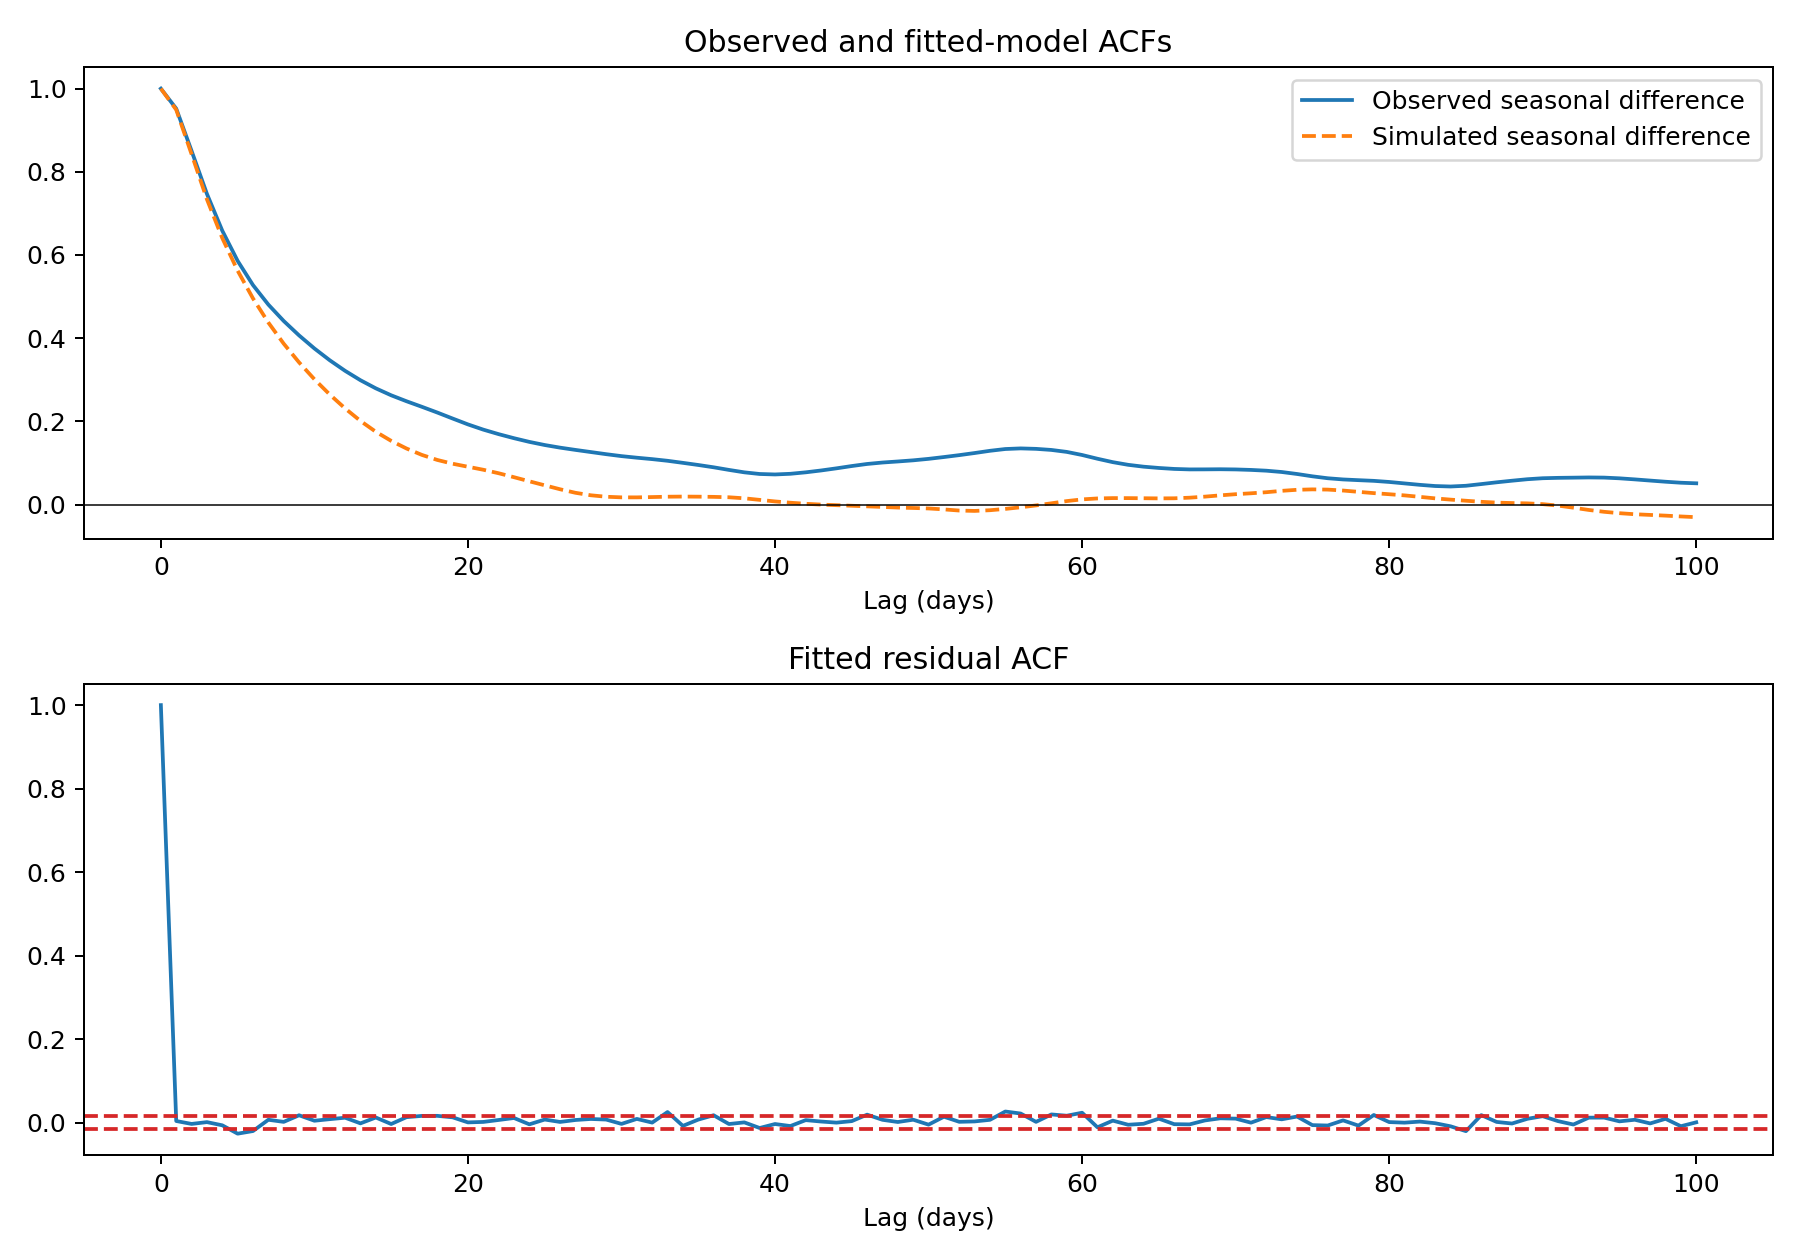
\includegraphics[width=0.95\linewidth]{problem2_nao_validation.png}
    \caption{Validation using a simulation from the fitted seasonal model.}
\end{figure}
\vspace{1em}

\item[$4^*$] an ARIMA$(p,1,q)$ process is effectively an ARMA$(p,q)$ process with a ``unit root'', meaning $\phi(z)=0$ for some $|z|=1$. Interpret the implication of this addition to the model in the spectral domain. How is the ARMA spectral density impacted? What are the downsides of such a design? Try and propose an extension of ARMA models in the same spirit, but that addresses your identified downside.
\par\vspace{0.5em}\textbf{Sol.}\par
For
\[
\phi(B)(1-B)X_t=\theta(B)Z_t,
\]
the formal spectral density is
\[
f_X(\lambda)=\frac{\sigma^2}{2\pi}
\frac{|\theta(e^{-i\lambda})|^2}
{|\phi(e^{-i\lambda})|^2|1-e^{-i\lambda}|^2}.
\]
Since $|1-e^{-i\lambda}|^2=4\sin^2(\lambda/2)\sim\lambda^2$ near zero,
the unit root creates a second-order pole at frequency zero. The expression is
not integrable there, reflecting the nonstationarity and unbounded variance of
the level process. Differencing removes this pole, but an integer difference
is rigid: it forces exactly this singularity and can overdifference data whose
low-frequency persistence is strong but not a unit root. Forecast uncertainty
for the level also grows without bound with the forecast horizon.

A natural extension is ARFIMA$(p,d,q)$,
\[
\phi(B)(1-B)^dX_t=\theta(B)Z_t,
\]
where $d$ need not be an integer. Its spectrum contains the factor
$|1-e^{-i\lambda}|^{-2d}$. For $0<d<1/2$ the process is stationary but has a
controlled singularity at zero and long-range dependence. Thus fractional
differencing preserves low-frequency persistence without imposing the full
nonstationary unit root.
\end{enumerate}

\newpage
\subsection*{Problem 3.}
Consider a stationary time series $\{Y_t\}$ with mean zero and covariance sequence given by
\[
\operatorname{Cov}(Y_t,Y_{t-h})=K(h)
=\frac{2e^{-\theta/2}\bigl(-\theta\cos(\pi h)+e^{\theta/2}\theta+2\pi h\sin(\pi h)\bigr)}{\theta^2+(2\pi h)^2}.
\]
Let's fit an ARMA process to this and see what is going on.
\begin{enumerate}[label=\arabic*.,leftmargin=*]
\item Write code to simulate draws from this process of length $n=1{,}000$ directly using the Cholesky factor of the covariance matrix. You are welcome to use built-in routines for the Cholesky factorization itself, but please otherwise write this code yourself.
\par\vspace{0.5em}\textbf{Sol.}\par
I used $\theta=6$. Define the Toeplitz covariance matrix
\[
\Gamma_{ij}=K(i-j),\qquad 1\leq i,j\leq 1000.
\]
Since $K$ is a covariance sequence, $\Gamma$ is non-negative definite. Its
Cholesky factorization is $\Gamma=LL'$. If
$\mathbf z\sim N(\mathbf0,I_{1000})$ and $\mathbf y=L\mathbf z$, then
\[
\mathbb E\mathbf y=\mathbf0,
\qquad
\operatorname{Cov}(\mathbf y)=LIL'=\Gamma.
\]
Thus the entries of $\mathbf y$ are one Gaussian draw with the required
covariance. The appendix constructs $\Gamma$, computes $L$, and generates the
draw directly in this way. A numerical diagonal adjustment of $10^{-12}$ was
used only to avoid roundoff problems in the factorization.
\vspace{1em}

\item Pick orders $p$ and $q$ (again, I suggest trying different combinations for max fun!) and fit an ARMA$(p,q)$ model to that simulation. Plot the implied ARMA ACF against the true ACF and comment on the patterns. You are again welcome to use a package for both fitting and obtaining the ARMA ACF.
\par\vspace{0.5em}\textbf{Sol.}\par
I chose $p=q=4$ as a compromise between flexibility near lag zero and avoiding
an unnecessarily high-order fit. A Whittle fit to the simulated series gave
\begin{align*}
\widehat{\boldsymbol\phi}
&=(.17383,-.26896,-.65793,.33627),\\
\widehat{\boldsymbol\theta}
&=(.44727,.37068,.90769,.16742),\\
\widehat\sigma^2&=.23108.
\end{align*}
The fitted ACF reproduces the sharp fall from lag 0 to lag 1 and is already
close to zero by lag 5. It also introduces small alternating correlations at
intermediate lags. These oscillations are needed because a finite rational
spectrum can only approximate the cusp of the true spectrum; the empirical
ACF itself has additional fluctuations from the single finite sample.

\begin{figure}[htbp]
    \centering
    \graphicspath{{png/}{STATS_Minor/701/HW2/png/}}
    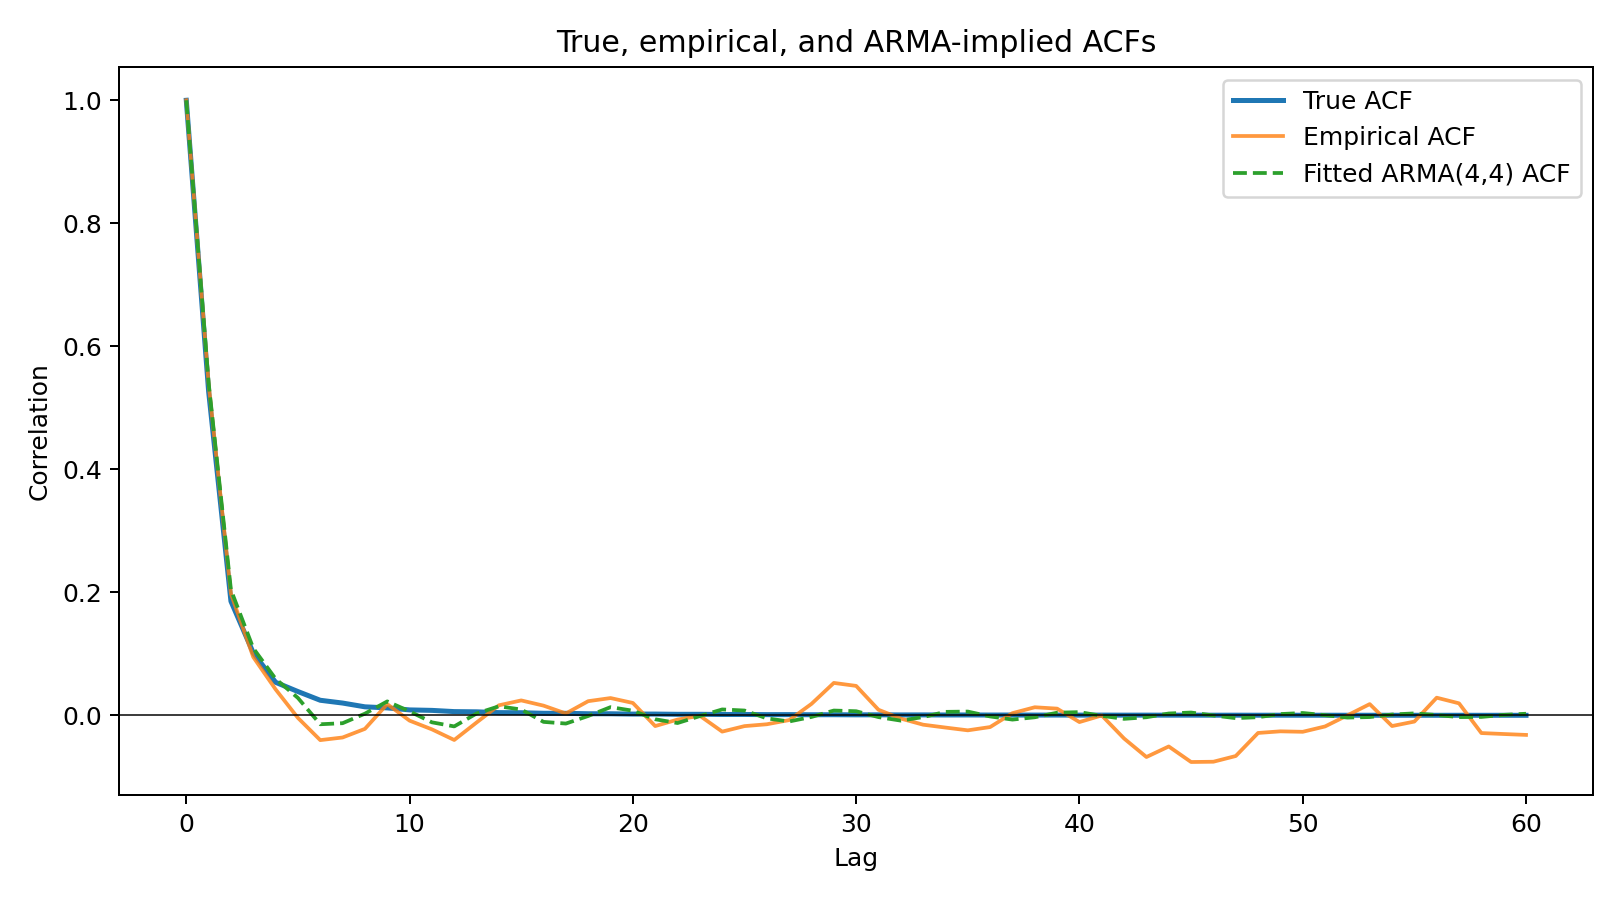
\includegraphics[width=0.9\linewidth]{problem3_acf_comparison.png}
    \caption{True, empirical, and fitted ARMA$(4,4)$ autocorrelations.}
\end{figure}
\vspace{1em}

\item[$3^*$.] Show that this $K(h)$ corresponds to a spectral density given by $S(\omega)=e^{-\theta|\omega|}$. Plot this true spectral density, and in the same plot also add the ARMA model-implied SDF using your fitted parameters. Comment on the quality of the fit and any specific issues you see.
\par\vspace{0.5em}\textbf{Sol.}\par
Using frequency in cycles per observation, $\omega\in[-1/2,1/2]$, the inverse
Fourier transform of the proposed density is
\begin{align*}
\int_{-1/2}^{1/2}e^{-\theta|\omega|}e^{2\pi ih\omega}\,d\omega
&=2\int_0^{1/2}e^{-\theta\omega}\cos(2\pi h\omega)\,d\omega\\
&=\frac{2e^{-\theta/2}}{\theta^2+(2\pi h)^2}
\left[-\theta\cos(\pi h)+2\pi h\sin(\pi h)
+e^{\theta/2}\theta\right]\\
&=K(h).
\end{align*}
Hence $S(\omega)=e^{-\theta|\omega|}$ is the spectral density corresponding
to $K$.

The time-series fit follows the overall decay away from frequency zero, but it
rounds off the cusp at zero and creates two artificial notches and shoulders
near frequencies $\pm .25$. Its root-mean-square log-spectral error over a
dense grid is $.11813$. These local artifacts are the frequency-domain version
of the small oscillations in the fitted ACF.

\begin{figure}[htbp]
    \centering
    \graphicspath{{png/}{STATS_Minor/701/HW2/png/}}
    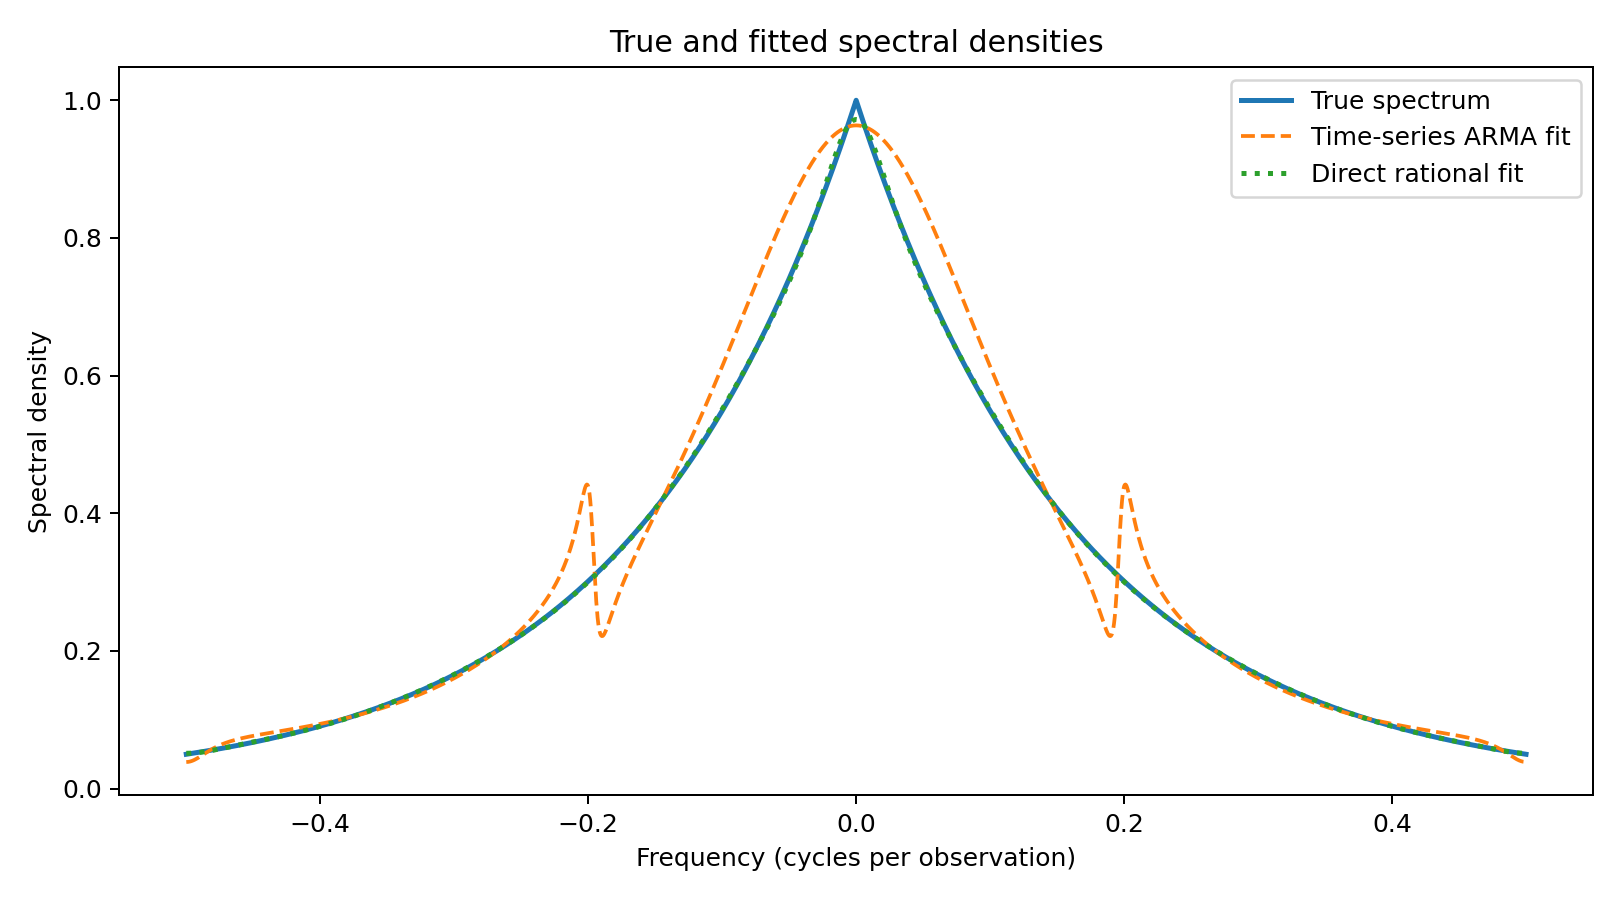
\includegraphics[width=0.9\linewidth]{problem3_spectrum_comparison.png}
    \caption{True spectrum, the fit to the simulated series, and the direct rational fit.}
\end{figure}
\vspace{1em}

\item[$4^*$.] Google around and choose an algorithm with a convenient package for fitting rational functions (you might look at the \textit{Remez} or \textit{AAA} algorithms, for example). Fit a rational function of the same order as your chosen ARMA process to directly to the true spectral density you verified in the last part, trying carefully to match the way that ARMA SDFs are parameterized. Compare your results with the fitted ARMA coefficients you obtained in 2 and discuss potential differences you observe.
\par\vspace{0.5em}\textbf{Sol.}\par
I used nonlinear rational least squares through
\texttt{scipy.optimize.least\_squares}. The fitted family was parameterized
exactly as an ARMA$(4,4)$ spectrum,
\[
S_{\mathrm{ARMA}}(\omega)
=\sigma^2\frac{|1+\sum_{j=1}^4\theta_je^{-2\pi ij\omega}|^2}
{|1-\sum_{j=1}^4\phi_je^{-2\pi ij\omega}|^2}.
\]
Reflection coefficients constrained the AR and MA polynomials to the stable
and invertible regions, and the criterion was least squares on the log
spectrum over $2{,}001$ equally spaced frequencies. The result was
\begin{align*}
\widetilde{\boldsymbol\phi}
&=(.28813,.68534,-.17504,-.02755),\\
\widetilde{\boldsymbol\theta}
&=(.31981,-.67572,-.18970,.02384),\\
\widetilde\sigma^2&=.22313.
\end{align*}
Its log-spectral root-mean-square error is $.00416$, far below $.11813$ for
the time-series fit. The two coefficient vectors differ because the direct fit
uses the exact target spectrum at every grid point, whereas the first fit sees
only one random sample and minimizes a Whittle likelihood based on its noisy
periodogram. Moreover, finite-order AR and MA factors can trade off while
producing similar spectral shapes. As Figure 5 shows, the direct fit is nearly
indistinguishable from the target except in a very small neighborhood of the
nondifferentiable cusp at zero.
\end{enumerate}

\clearpage
\appendix
\section{Python code}
The scripts read \texttt{code/nao.csv} relative to the HW2 directory and save
all figures in \texttt{png/}. They use NumPy, pandas, SciPy, Matplotlib, and
statsmodels.

\subsection{Problem 2}
\lstinputlisting[language=Python]{code/problem2.py}

\clearpage
\subsection{Problem 3}
\lstinputlisting[language=Python]{code/problem3.py}

\end{document}
